% tikz flowchart

% listing of script
\lstinputlisting[style= Matlab-editor,basicstyle = \mlttfamily,
  caption=Exercise 6 script]{Week_2_master/exercise6.m}

% four plots as specified
\begin{figure}[H]
\centering
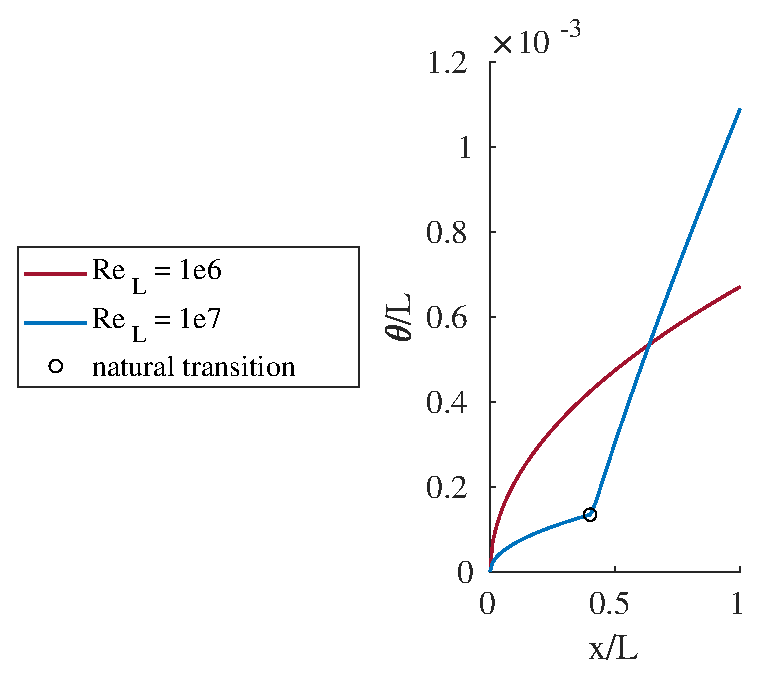
\includegraphics[scale=0.70]{graphs/e6g1.eps}
\caption{}
\label{e6g1}
\end{figure}

\begin{figure}[H]
\centering
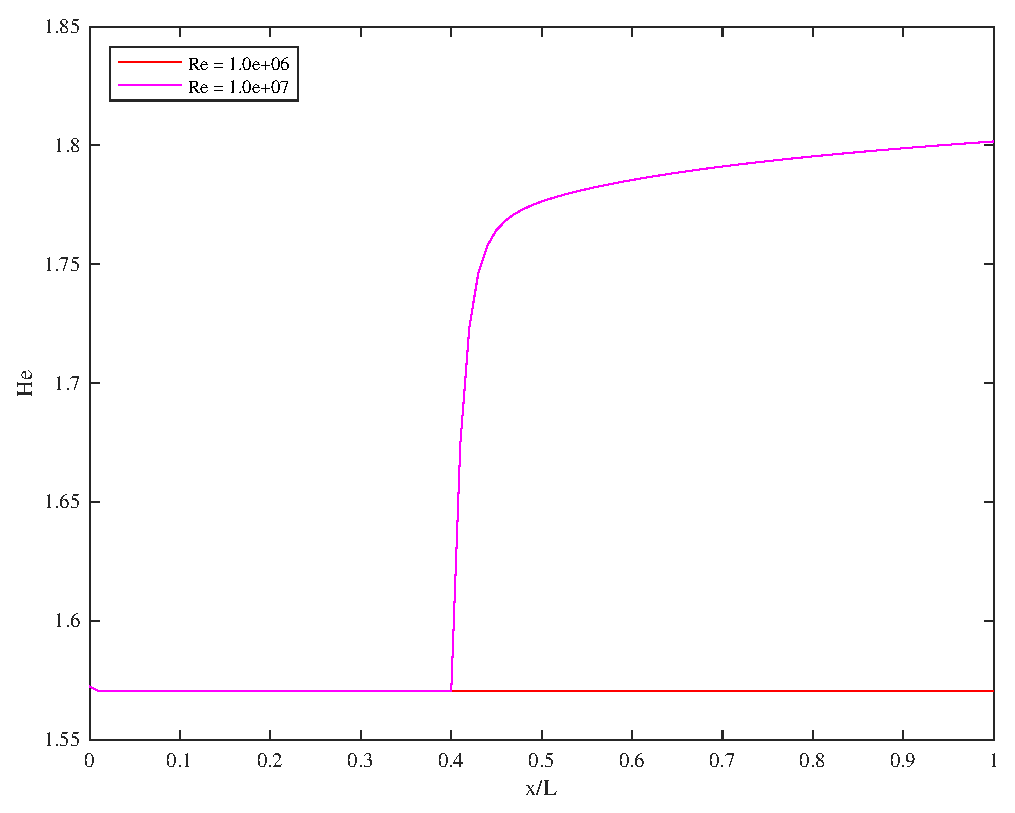
\includegraphics[scale=0.70]{graphs/e6g2.eps}
\caption{}
\label{e6g2}
\end{figure}

\begin{figure}[H]
\centering
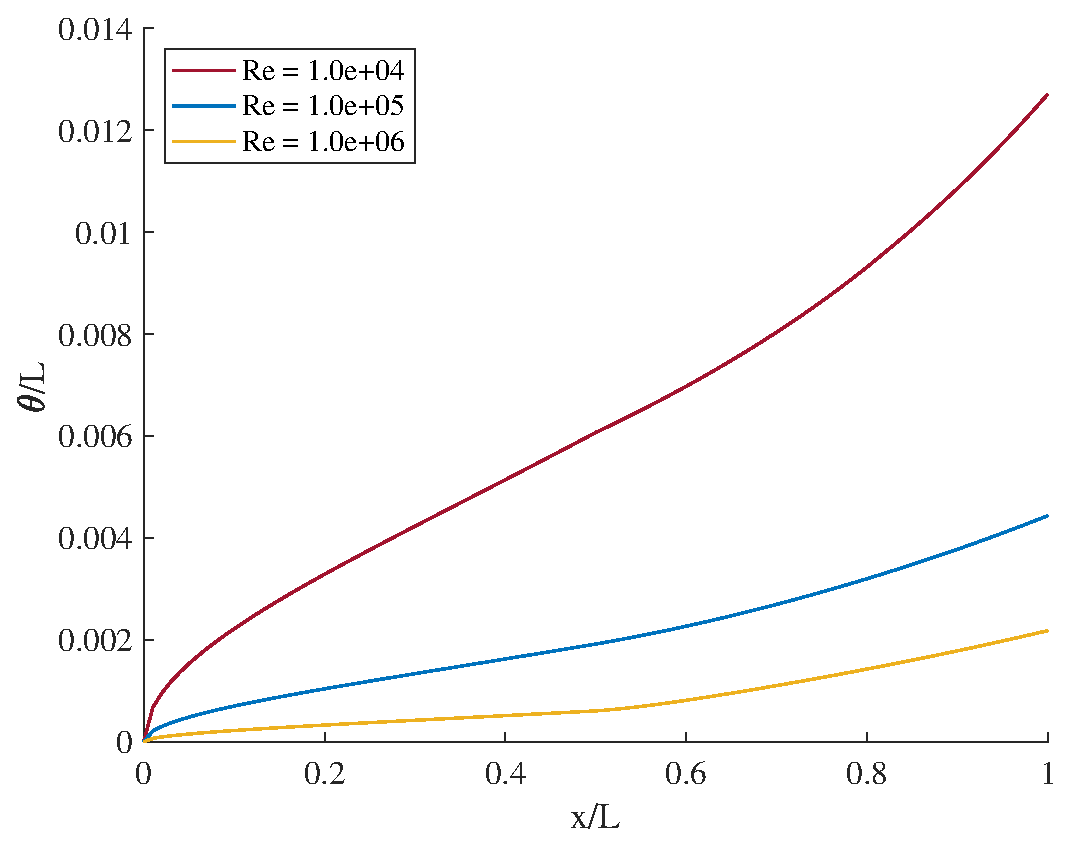
\includegraphics[scale=0.70]{graphs/e6g3.eps}
\caption{}
\label{e6g3}
\end{figure}

\begin{figure}[H]
\centering
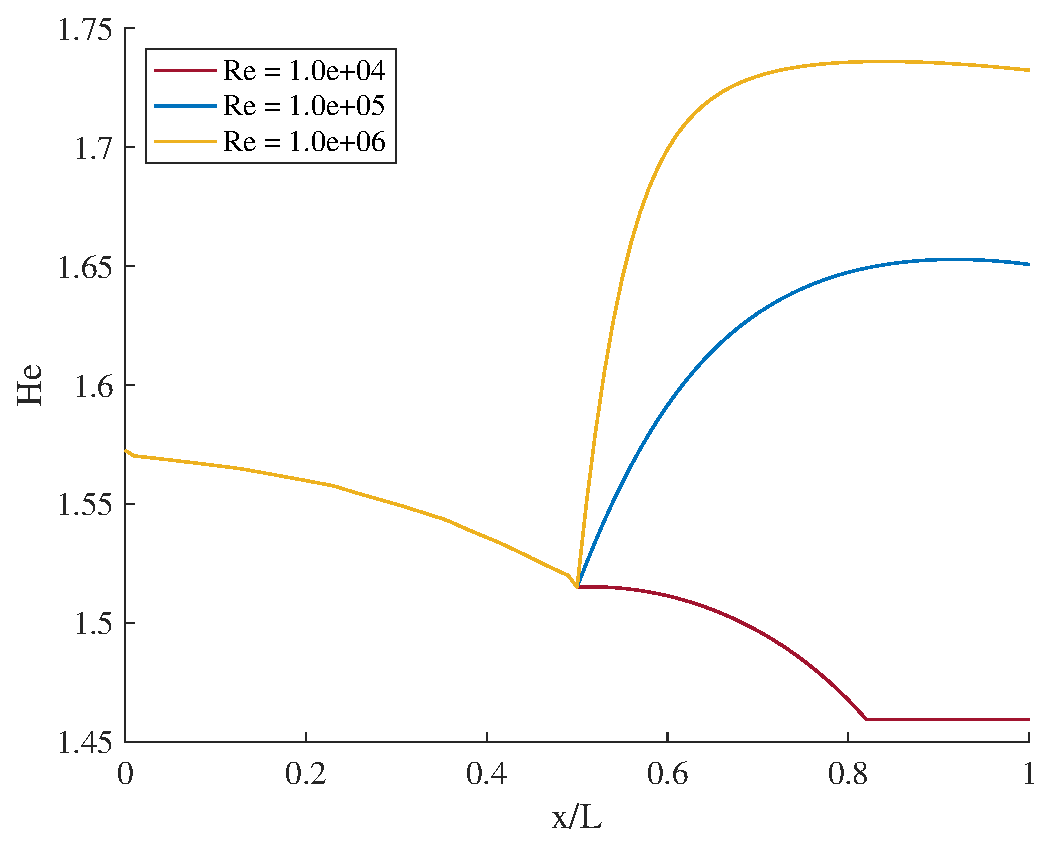
\includegraphics[scale=0.70]{graphs/e6g4.eps}
\caption{}
\label{e6g4}
\end{figure}

\tikzset{every picture/.style={line width=0.75pt}} %set default line width to 0.75pt        

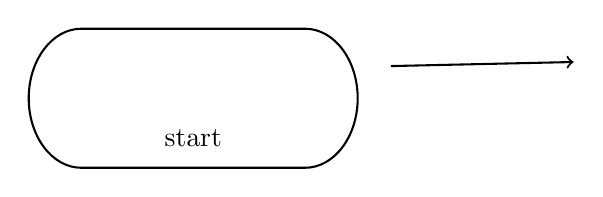
\begin{tikzpicture}[x=0.75pt,y=0.75pt,yscale=-1,xscale=1]
%uncomment if require: \path (0,406); %set diagram left start at 0, and has height of 406

%Flowchart: Terminator [id:dp442991202759064] 
\draw   (83.36,86) -- (191.14,86) .. controls (205.15,86) and (216.5,101) .. (216.5,119.5) .. controls (216.5,138) and (205.15,153) .. (191.14,153) -- (83.36,153) .. controls (69.35,153) and (58,138) .. (58,119.5) .. controls (58,101) and (69.35,86) .. (83.36,86) -- cycle ;
%Straight Lines [id:da10986730772092312] 

\draw [->](232.5,104) -- (320.5,102.04) ;
%\draw [shift={(322.5,102)}, rotate = 538.73] [color={rgb, 255:red, 0; green, 0; blue, 0 }  ][line width=0.75]    (10.93,-3.29) .. controls (6.95,-1.4) and (3.31,-0.3) .. (0,0) .. controls (3.31,0.3) and (6.95,1.4) .. (10.93,3.29)   ;

% Text Node
\draw (122,133) node [anchor=north west][inner sep=0.75pt]   [align=left] {start};


\end{tikzpicture}

% critical velocity gradient as specified